\chapter{Background}
\label{ch:background}

This chapter introduces the fundamental concepts and technologies
that form the basis of the architectural analysis process developed
in this thesis. It begins by defining \textbf{software dependencies}
and their representation through \textbf{graphs}, then examines
traditional \textbf{static analysis} approaches, and finally details
the parsing mechanisms and the \textbf{Tree-sitter} framework
utilized in this work.

\section{Software Dependencies}
\label{sec:software_dependencies}

In software engineering, a \textbf{dependency} exists when a
component requires the presence or functionality of another component
to perform its task or to compile correctly
\cite{martin_clean_2018}. Managing these dependencies is
arguably one of the most critical aspects of software design. It is
directly related to the concepts of \textbf{coupling} (the degree of
interdependence between software modules) and \textbf{cohesion} (the
degree to which elements inside a module belong together). A
well-architected system typically aims for \textit{high cohesion} and
\textit{low coupling}, ensuring that components can be maintained,
tested, and extended in isolation without triggering cascading
changes across the entire codebase.

Dependencies in modern programming languages can manifest in several
distinct forms, each carrying a different weight and architectural
implication. They can be broadly categorized as shown in Table
\ref{tab:dependency_types}.

\begin{table}[ht]
  \small
  \centering
  % "1\textwidth"
  \renewcommand{\arraystretch}{1.5}
  \begin{tabularx}{\textwidth}{|p{0.2\textwidth}|X|}
    \hline
    \textbf{Category} & \textbf{Examples and Architectural Implications} \\
    \hline
    \textbf{Structural / Compositional} & \textbf{Aggregation \&
    Composition:} A type declares a field/property of another type
    (e.g., \texttt{Car} has an \texttt{Engine}).\newline
    \textbf{Type Aliases:} Defining a new name for an existing type
    (\texttt{typedef}, \texttt{using}).\newline
    \textbf{Generic Bounds:} Restricting a generic type parameter
    (e.g., \texttt{T extends B}).\newline
    \textit{Implication:} Alters the physical memory layout and
    fundamentally ties the data structures together. \\
    \hline
    \textbf{Inheritance / Realization} & \textbf{Class Extension:} A
    class derives from a base class.\newline
    \textbf{Interface Implementation:} A class fulfills an interface
    contract.\newline
    \textbf{Trait Mixins:} Including behavior from traits (e.g., in
    Rust or Scala).\newline
    \textit{Implication:} The strongest form of coupling
    (\textit{IS-A} relationship). The child is inextricably tied to
    the parent's lifecycle and public contract. \\
    \hline
    \textbf{Behavioral / Control Flow} & \textbf{Method Invocations:}
    Calling a function or method.\newline
    \textbf{Instantiations:} Creating a new object (\texttt{new B()}).\newline
    \textbf{Field Access:} Reading or writing to another class's
    properties.\newline
    \textbf{Signature Types:} Using a type as a formal parameter or
    return type.\newline
    \textbf{Exception Handling:} Catching a specific exception type.\newline
    \textit{Implication:} Dictates runtime behavior and creates
    strict compile-time bonds, without altering structural memory layouts. \\
    \hline
  \end{tabularx}
  \caption{Taxonomy of software dependencies extracted via static analysis.}
  \label{tab:dependency_types}
\end{table}

Furthermore, dependency tracking must distinguish between
\textbf{static} and \textbf{dynamic} analysis. \textbf{Static
analysis} examines the source code strictly at rest, extracting only
the explicit relationships defined by the syntax and the type system.
Conversely, \textbf{dynamic dependencies}, such as those introduced
by reflection, dependency injection containers, late binding
(polymorphism), or features like Python's \texttt{eval()}, manifest
their true target only during program execution
\cite{horwitz_interprocedural_1988}. Because static analysis cannot
reliably predict the runtime state, it focuses exclusively on the
declared, compile-time architecture. This thesis is strictly scoped
to the extraction and modeling of \textit{static} dependencies.

\section{Software Quality and Code Smells}
\label{sec:smells}

The concept of a "smell" was popularized by Martin Fowler in the
context of software engineering \cite{fowler_refactoring_2013} to
indicate a symptom of possible deterioration in software quality. A
smell is not necessarily a bug; rather, it is a surface indication
that usually corresponds to a deeper problem in the system's design
or maintainability. Left unaddressed, smells accumulate and manifest
as Technical Debt \cite{cunningham_wycash_1992}, a metaphor
describing the implied cost of additional rework caused by choosing
an easy (often flawed) solution now instead of using a better
approach that would take longer.

Smells are generally categorized by their scope and impact:
\begin{itemize}
  \item \textbf{Code Smells:} These are localized indicators of poor
    programming practices, usually confined to a single method or
    class. Examples include \textit{Long Method}, \textit{Large
    Class}, or \textit{Long Parameter List}. Because they are local,
    they can often be detected through simple syntactic analysis and
    resolved through standard refactoring techniques without
    affecting the rest of the system.
  \item \textbf{Architectural Smells:} Unlike code smells,
    architectural smells \cite{garcia_identifying_2009} are
    global issues that affect the high-level structure of the
    software, such as the organization of modules, the interactions
    between packages, and the overall dependency graph. They are
    significantly more difficult to identify and correct because they
    require a holistic understanding of the entire system's
    architecture. Correcting an architectural smell often involves
    deep, cross-cutting modifications that can impact multiple
    components simultaneously.
\end{itemize}

\section{Dependency Graphs and Architectural Representation}
\label{sec:dependency_graphs}

To systematically analyze, navigate, and reason about software
architecture and its associated smells, the extracted dependencies
are typically modeled using \textbf{Graph Theory}. The analysis
process often relies on distinguishing between a \textit{Component
Graph} and a \textit{Dependency Graph}.

\subsection{Component and Dependency Graphs}

A \textbf{Component Graph} represents the hierarchical containment
and physical organization of the source code. It is defined as a directed graph:
\[
  G_c = (V, E_c)
\]
where $V$ is the set of vertices representing software components
(e.g., a package, a class, or a method), and $E_c \subseteq V \times
V$ is the set of directed edges representing strict containment
relationships, such that an edge $(u, v) \in E_c$ indicates that
component $u$ contains component $v$ (e.g., a method defined inside a class).

A \textbf{Dependency Graph} extends the component graph by modeling
the semantic interactions between these components. It is defined as
a multigraph:
\[
  G = (V, E) \quad \text{with} \quad E = E_c \cup E_d
\]
The set $E_d$ contains all the logical dependencies extracted from
the code. A dependency fundamentally exists whenever a piece of code
(Component A) cannot function, compile, or execute without the
presence of another (Component B).

\begin{figure}[htpb]
  \centering
  \includegraphics[width=\textwidth]{images/background/dep-graph-example.png}
  \caption{Small example of a Dependency Graph}
  \label{fig:example_dependency_graph}
\end{figure}

In the context of source code, the \textbf{granularity} of these
vertices can vary. They can represent high-level architectural
boundaries, file-level modules, or fine-grained code constructs (such
as classes, interfaces, or individual functions). The edges are
intrinsically \textbf{directed}: if class \texttt{A} calls a method
of class \texttt{B}, the edge points from \texttt{A} to \texttt{B},
establishing a dependency vector that indicates \texttt{A} is
vulnerable to changes in \texttt{B}, but not necessarily vice versa.
An illustrative example of a real-world software dependency graph is
provided in Figure \ref{fig:example_dependency_graph}, visually
demonstrating how components interlock.

\subsection{Dependency Smells}
Mapping source code to a graph structure provides a powerful
mathematical foundation to evaluate the system's health and
automatically detect specific Architectural Smells, often referred
to as \textbf{Dependency Smells}. The presence of these
configurations in the graph usually indicates a violation of core
design principles (such as SOLID, high cohesion, or loose coupling).
Notable dependency smells include \cite{noauthor_arcan_nodate}:

\begin{itemize}
  \item \textbf{Cyclic Dependency:} The most notorious anomaly occurs
    when two or more components are linked by circular dependency
    relationships, forming a cycle in the graph. This violates the
    Acyclic Dependencies Principle, rendering the involved components
    inseparable, impossible to test in isolation, and prone to
    infinite recursion. A healthy architectural dependency graph is
    generally expected to form a \textbf{Directed Acyclic Graph (DAG)}.

    Consider the Java example in Listing \ref{lst:cyclic_dep}, where
    three services (\texttt{ServiceA}, \texttt{ServiceB}, and \texttt{ServiceC})
    depend on each other in a closed loop. This generates a cycle in
    the dependency graph, as visually represented in Figure
    \ref{fig:cyclic_dependency}.

\begin{lstlisting}[language=Java,caption={Example of a Cyclic Dependency involving three Java services.},label={lst:cyclic_dep}]
// In ServiceA.java
public class ServiceA {
    private ServiceB b = new ServiceB();
}

// In ServiceB.java
public class ServiceB {
    private ServiceC c = new ServiceC();
}

// In ServiceC.java
public class ServiceC {
    private ServiceA a = new ServiceA();
}
\end{lstlisting}

    \begin{figure}[H]
      \centering
      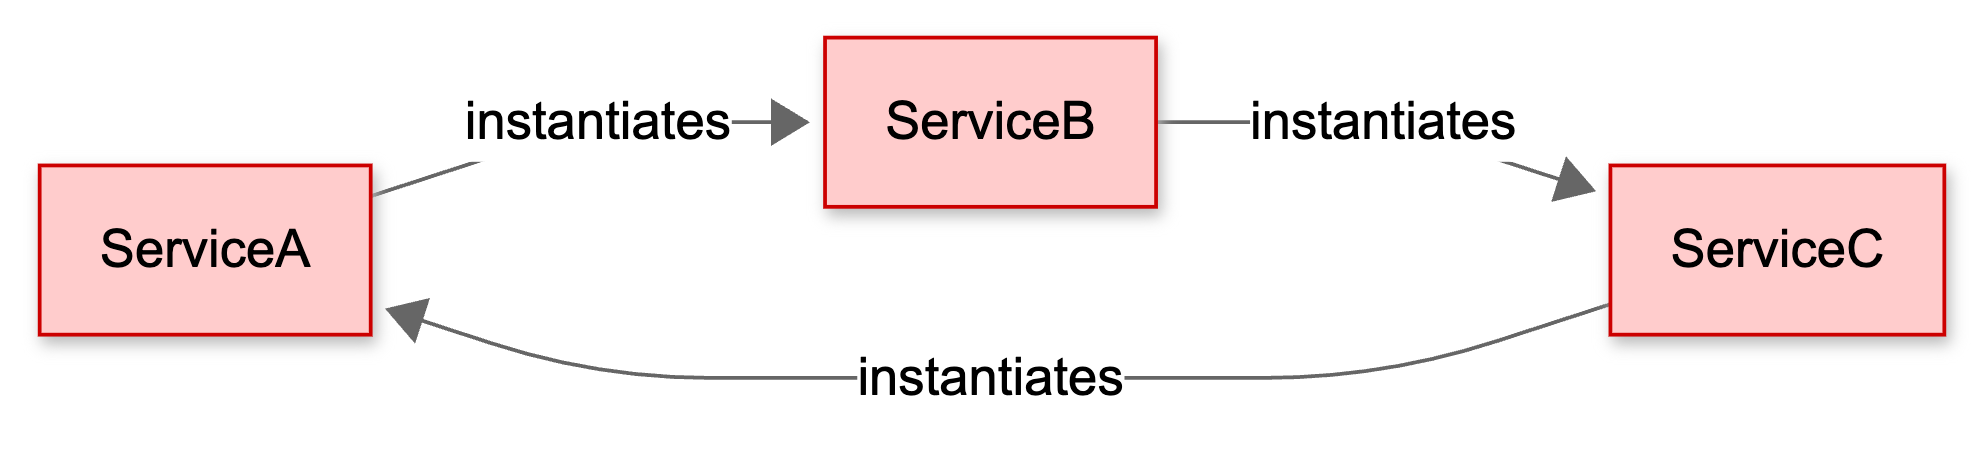
\includegraphics[width=0.5\textwidth]{images/background/cyclic_dependency.png}
      \caption{Dependency graph resulting from a Cyclic Dependency smell.}
      \label{fig:cyclic_dependency}
    \end{figure}
  \item \textbf{Unstable Dependency:} This occurs when a stable, core
    component depends on one or more highly unstable, frequently
    changing components. This configuration violates the Stable
    Dependencies Principle \cite{martin_clean_2018},
    exposing central components to frequent variations and increasing
    the risk of cascading failures.
  \item \textbf{Hub-Like Dependency:} A component assumes a role of
    excessive centrality, exhibiting a very high number of both
    incoming and outgoing dependencies. Such "hub" components become
    critical bottlenecks, concentrating heterogeneous
    responsibilities and severely limiting the modularity and
    independent evolution of the system.
  \item \textbf{Deep Hierarchy:} An inheritance hierarchy that is
    excessively deep, where components at the bottom depend on a long
    chain of supertypes. This increases system complexity and makes
    the behavior of child classes difficult to predict.
  \item \textbf{Wide Hierarchy:} An inheritance hierarchy that is
    excessively broad, with a single parent class having an unusually
    large number of direct subclasses. This often indicates poor
    intermediate abstraction or an incomplete decomposition of responsibilities.
  \item \textbf{Cyclic Hierarchy:} A critical structural error where
    an inheritance hierarchy forms a cycle (e.g., a supertype
    directly or indirectly inheriting from its own subtype). This
    breaks the fundamental \textit{IS-A} relationship paradigm and
    can lead to severe compilation or runtime errors.
\end{itemize}

\section{Traditional Static Analysis and Tooling}
\label{sec:traditional_static_analysis}

Extracting structural information from source code requires robust
static analysis tools. Traditionally, this process relies heavily on
\textbf{compiler front-ends}, such as Clang for C/C++ or Roslyn for
C\# \cite{lattner_llvm_2004}. A compiler front-end typically performs:
\begin{enumerate}
  \item \textbf{Lexical Analysis (Tokenization):} Converting text
    into a stream of tokens.
  \item \textbf{Syntactic Analysis (Parsing):} Grouping tokens into
    grammatical structures.
  \item \textbf{Semantic Analysis:} Type checking and symbol resolution.
\end{enumerate}

Because these tools must generate executable code, they possess a
mathematically sound and exhaustive understanding of the language's
semantics. However, this deep integration is also their primary
\textit{limitation}: they are inherently \textbf{coupled to a single
programming language}, its specific version, and its build ecosystem.

\subsection{Intermediate Representations (IR) and the $M \times N$ Problem}
Developing a cross-language analysis system using language-specific
tools forces engineers to integrate disparate compiler
front-ends, each with its own output format, terminology,
and execution environment. If the system must support $M$ source
languages and $N$ analysis tools (or back-ends), each tool must be
individually integrated with each language's front-end, resulting in
$M \times N$ separate integration efforts. As both $M$ and $N$ grow,
this combinatorial complexity becomes unsustainable.

Modern compiler architectures, such as LLVM \cite{lattner_llvm_2004},
solve this problem by introducing an
\textbf{Intermediate Representation (IR)}: a standardized,
language-agnostic data structure that sits between the front-end
(which parses the source code) and the back-end (which performs
analysis or generates machine code). Each language requires only one
front-end that translates source code into the IR, and each tool
requires only one back-end that consumes the IR. The total number of
components is thus reduced from $M \times N$ to $M + N$. This
architectural transition is visually illustrated in Figure
\ref{fig:mxn_problem}.

\begin{figure}[H]
  \centering
  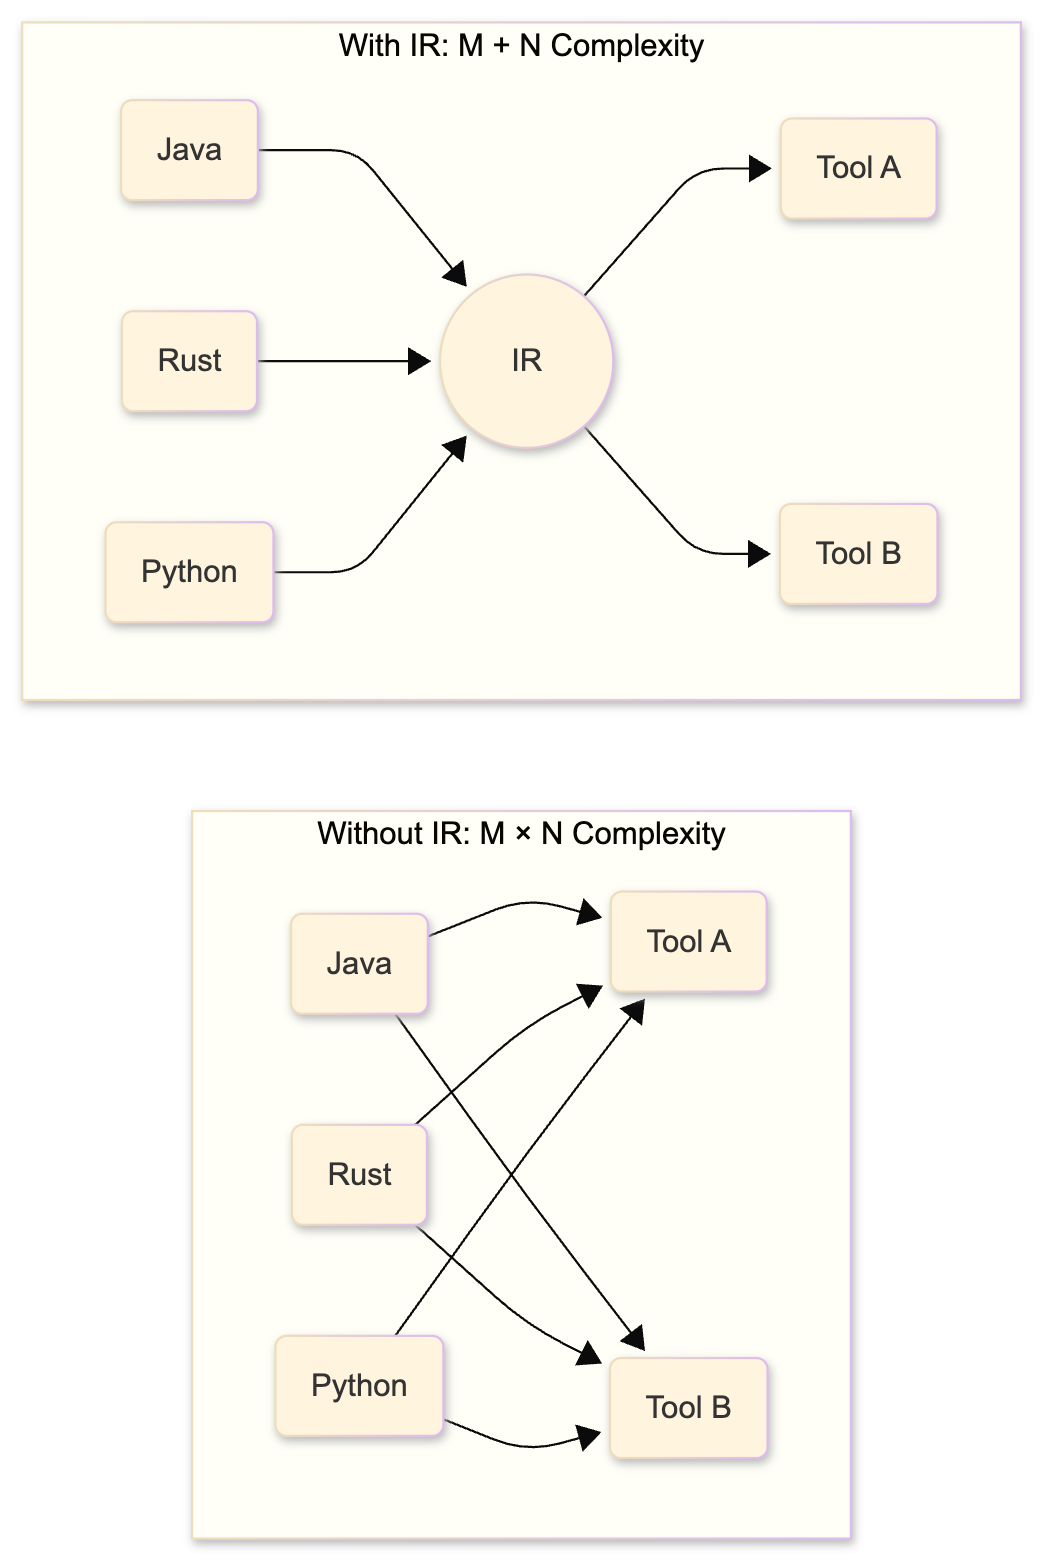
\includegraphics[width=\textwidth]{images/background/mxn_problem.png}
  \caption{Comparison between the $M \times N$ combinatorial
  explosion and the linear $M + N$ complexity achieved by introducing an IR.}
  \label{fig:mxn_problem}
\end{figure}

While LLVM uses a low-level IR focused on executable instructions,
architectural analysis requires a high-level, structural
representation. The same $M \times N$ decoupling principle applies to
this domain in two concrete ways:

\begin{itemize}
  \item \textbf{Internal decoupling:} Even within a single analysis
    tool, the pipeline contains multiple language-agnostic phases
    (name resolution, graph construction, export, visualization).
    Without an IR, each of these phases would need to handle the
    syntactic details of every supported language. With a shared IR,
    only the extraction phase is language-specific; all subsequent
    phases operate on a single, unified data model.
  \item \textbf{Ecosystem reuse:} A well-defined architectural IR can
    be consumed by multiple independent tools (e.g., architectural
    smell detectors, refactoring assistants, dependency auditors)
    without each tool reimplementing its own extraction logic for each
    language.
\end{itemize}

Designing a universal IR that captures the architectural semantics of
heterogeneous languages, without descending into low-level memory
layouts, is the core theoretical foundation required to build a truly
scalable, language-agnostic dependency extractor.

In recent years, protocols like the \textbf{Language Server Protocol
(LSP)} have attempted to standardize how development environments
interact with language-specific analyzers \cite{microsoft_lsp_spec}.
By standardizing the communication JSON-RPC interface, an IDE can
interact with any language server to request symbol definitions or
references. However, LSP is fundamentally designed for
\textbf{interactive, query-based use cases} (e.g., hovering over a
  variable to see its type, or requesting "find references" for a
specific symbol within an open file). Constructing a global
dependency graph of an entire repository requires a
\textbf{batch-processing approach}. Attempting to use LSP for this
purpose would involve artificially spoofing thousands of "find
references" queries across every symbol in every file, a process that
is highly stateful, incredibly slow, and simply suboptimal for
full-scale architectural extraction.

\section{Parsing Technologies and Tree-sitter}
\label{sec:parsing_and_treesitter}

The foundation of any static analysis tool is the \textbf{parser},
which translates raw source text into a structured tree
representation. Before the widespread adoption of parser generators,
some code analysis tools relied on pattern matching and
\textbf{regular expressions} to extract structural information from
source files. However, according to the Chomsky hierarchy
\cite{chomsky_three_1956}\cite{jager_formal_2012}, regular
expressions are formally incapable of correctly parsing context-free
languages, which encompass all modern programming languages. They
cannot reliably track nested structures, such as matched parentheses
or nested code blocks \cite{aho_compilers_2007}, leading to brittle
tools that break on complex formatting or edge cases.

When analyzing source code properly, parsers generally produce one of
two tree variants:
\begin{itemize}
  \item \textbf{Abstract Syntax Tree (AST):} Abstracts away the
    syntactical details that do not affect the program's logic, such
    as punctuation, whitespace, and comments, focusing only on the
    semantics (e.g., a "binary operation" node instead of explicitly
    storing the '+' token). This makes it highly suitable for
    compiler back-ends.
  \item \textbf{Concrete Syntax Tree (CST):} Represents the exact,
    unaltered syntactic structure of the source text, maintaining a
    strict one-to-one mapping with the original file. It includes all
    tokens, whitespace, and formatting, making it ideal for tooling
    that requires exact code correspondence, such as linters,
    formatters, and architectural analyzers.
\end{itemize}

\subsection{The Tree-sitter Framework}
To achieve high-performance, language-agnostic parsing, this project
utilizes \textbf{Tree-sitter} \cite{brunsfeld_treesitter_2018}.
Tree-sitter is a modern, generic parser generator that builds fast,
robust CSTs. It generates parsers from formal grammars written in a
Domain Specific Language (DSL) based on JavaScript.

One of the most defining characteristics of Tree-sitter is its vibrant,
community-driven ecosystem. Rather than relying on a centralized team
to build and maintain parsers, the ecosystem is heavily supported by
the open-source community. Today, there are robust, production-ready
parsers available for virtually all modern programming languages.

A fascinating side effect of this community-driven development is a
phenomenon of \textit{structural convergence}. When developers write a
Tree-sitter grammar for a new language, they frequently draw
inspiration from existing, well-established grammars (such as those
for C, Java, or Python). This cross-pollination naturally leads to a
shared structural ``DNA'' across different languages' syntax trees.
Naming conventions for AST nodes, hierarchical nesting rules, and
overall structural layouts end up being surprisingly similar, even for
languages with vastly different paradigms. As will be extensively
discussed in Chapter \ref{ch:extraction}, this emerging structural
similarity is the fundamental enabler of our framework. It allows us
to abstract away syntactic peculiarities and identify overarching
architectural components in a completely language-agnostic manner.

Under the hood, the generated parsers are implemented in C to
guarantee maximum performance and portability. Because they adhere to
the standard C Application Binary Interface (ABI), Tree-sitter
exposes a uniform API and provides native bindings for numerous
high-level languages, including Rust, Go, Java, and Python.

\subsubsection{Parsing and Navigation}

Using Tree-sitter within a Rust ecosystem requires initializing a
\texttt{Parser} instance and binding it to a specific language grammar
(such as \texttt{tree-sitter-rust} or \texttt{tree-sitter-java}).
Once configured, the parser consumes the raw source code string and
produces the Concrete Syntax Tree (CST).

Unlike traditional parsers that generate heavyweight, deeply nested
object hierarchies in memory, Tree-sitter's CST is backed by an
efficient C structure. To interact with it, static analyzers must
navigate this tree. Doing so via standard recursive object visits
could trigger stack overflows or incur severe heap allocation overhead
on massive codebases. To solve this, Tree-sitter provides the
\textbf{TreeCursor}.

The \texttt{TreeCursor} allows stateful, allocation-free traversal of
the syntax tree using imperative movements. Because the cursor mutates
its internal state \textit{in place} rather than allocating new node
objects at each step, it guarantees zero-allocation iteration over
arbitrarily large trees. Table \ref{tab:treecursor_methods} summarizes
the primary methods exposed by the cursor.

\begin{table}[ht]
  \footnotesize
  \centering
  \begin{tabularx}{\linewidth}{|l|X|l|}
    \hline
    \textbf{Cursor Method} & \textbf{Description} & \textbf{Returns} \\
    \hline
    \texttt{goto\_first\_child()} & Moves the cursor down to the
    first child of the current node. & \texttt{bool} \\
    \texttt{goto\_next\_sibling()} & Moves the cursor right to the
    next sibling of the current node. & \texttt{bool} \\
    \texttt{goto\_parent()} & Moves the cursor up to the parent of
    the current node. & \texttt{bool} \\
    \texttt{node()} & Retrieves the \texttt{Node} object currently
    pointed to by the cursor. & \texttt{Node} \\
    \texttt{field\_name()} & Returns the field name associated with
    the current node, if any. & \texttt{Option<\&str>} \\
    \hline
  \end{tabularx}
  \caption{Key methods provided by the \texttt{TreeCursor} API for
  stateful CST navigation.}
  \label{tab:treecursor_methods}
\end{table}

This uniform access mechanism is completely agnostic to the underlying
programming language. In our framework, the extraction phase relies
heavily on combining \texttt{goto\_first\_child()} and
\texttt{goto\_next\_sibling()} within loops to systematically crawl
through all components of a file. At any position, the cursor exposes
the current \texttt{Node}, allowing the analyzer to extract structural
metadata (via \texttt{node.kind()}) or the raw source string (via
\texttt{node.utf8\_text()}).
\\\\
Listing \ref{lst:tree_sitter_parsing} illustrates the complete pipeline:
from parser initialization to the stateful traversal of the resulting
tree, mimicking the pattern used heavily during the analysis phase of
our prototype.

\begin{lstlisting}[language=Rust,caption={Complete example of parsing source code and navigating the CST using Tree-sitter in Rust.},label={lst:tree_sitter_parsing}]
use tree_sitter::Parser;

// 1. Initialize the parser and set the target language
let mut parser = Parser::new();
parser.set_language(tree_sitter_java::language())
      .expect("Error loading Java grammar");

// 2. Parse the source code into a Concrete Syntax Tree
let source_code = b"class Main { int x; }";
let tree = parser.parse(source_code, None).unwrap();

// 3. Initialize the TreeCursor at the root node
let mut cursor = tree.root_node().walk();

// 4. Navigate the tree statefully without allocating memory
if cursor.goto_first_child() {
    loop {
        let node = cursor.node();
        println!("Node kind: {}", node.kind());

        if let Ok(text) = node.utf8_text(source_code) {
            println!("Text: {}", text);
        }

        // Move to the next sibling, or break if there are no more
        if !cursor.goto_next_sibling() {
            break;
        }
    }
    // Return to the parent scope
    cursor.goto_parent();
}
\end{lstlisting}

\subsubsection{Advantages over Traditional Generators}
Tree-sitter was selected over traditional parser generators (like
ANTLR, Bison, or Yacc) \cite{ortin_empirical_2022} for several
architectural reasons:

\begin{itemize}
  \item \textbf{Performance and Algorithm:} Tree-sitter uses a
    \textbf{Generalized LR (GLR)} parsing algorithm. Being a
    bottom-up parser (specifically LR(1)), it is generally faster and
    more efficient than top-down parsers like ANTLR's Adaptive LL(*).
    The time complexity for parsing is primarily bounded to $O(n)$,
    making it highly suitable for analyzing massive codebases.
  \item \textbf{Advanced Error Recovery:} When encountering a syntax
    error, Tree-sitter does not halt. Instead, it utilizes
    \texttt{ERROR} or \texttt{MISSING} nodes to bypass the anomaly
    and successfully parse the remainder of the file. This makes it
    incredibly robust for analyzing code under development.
  \item \textbf{Decoupling of Grammar and Code:} Tools like Bison and
    Yacc often require developers to mix executable C/C++ code
    directly into the grammar definitions (Syntax-Directed
    Translation). While powerful for compiling, this makes the
    grammar practically impossible to port to other languages.
    Conversely, Tree-sitter enforces a strict separation: the grammar
    only defines syntax, while the application (in our case, the Rust
    analyzer) queries the resulting tree.
\end{itemize}

\section{Name Resolution and Lexical Scoping}
\label{sec:name_resolution}

Extracting the syntax tree is only the first step in constructing a
dependency graph. The subsequent, and often significantly more
complex challenge, is \textbf{name resolution} (or symbol
resolution). Knowing syntactically that a class uses an identifier
named \texttt{B} is insufficient; the analyzer must determine
\textit{exactly which concrete type} \texttt{B} refers to within the
global project scope, distinguishing it from other types that might
share the same name in different modules.

This resolution process depends heavily on \textbf{lexical scoping}
rules, which dictate the visibility and lifetime of identifiers based
on their physical placement within the source code blocks
\cite{scott_programming_2016}. Scopes are typically
hierarchical: an inner scope (like a method body) can access
identifiers from its outer scope (like the class body or the global
namespace). Complicating matters is the concept of
\textbf{shadowing}, where a local variable might mask a global type
with the same name.

To correctly resolve a reference, static analyzers typically simulate
a bottom-up search (or "scope climbing"). As illustrated in the Java
snippet in Listing \ref{lst:scope_climbing} and its corresponding
diagram in Figure \ref{fig:scope_climbing}, when the analyzer
encounters the identifier \texttt{value} inside the \texttt{if} block,
it first checks the immediate block scope. Not finding it, it climbs
up to the method scope, and finally to the class scope, where the
declaration is matched.

\begin{lstlisting}[language=Java,caption={A simple Java class illustrating nested scopes.},label={lst:scope_climbing}]
public class Outer {
    int value; // Declaration matched at Class Scope
    void method() {
        if (true) {
            System.out.println(value); // Reference
        }
    }
}
\end{lstlisting}

\begin{figure}[H]
  \centering
  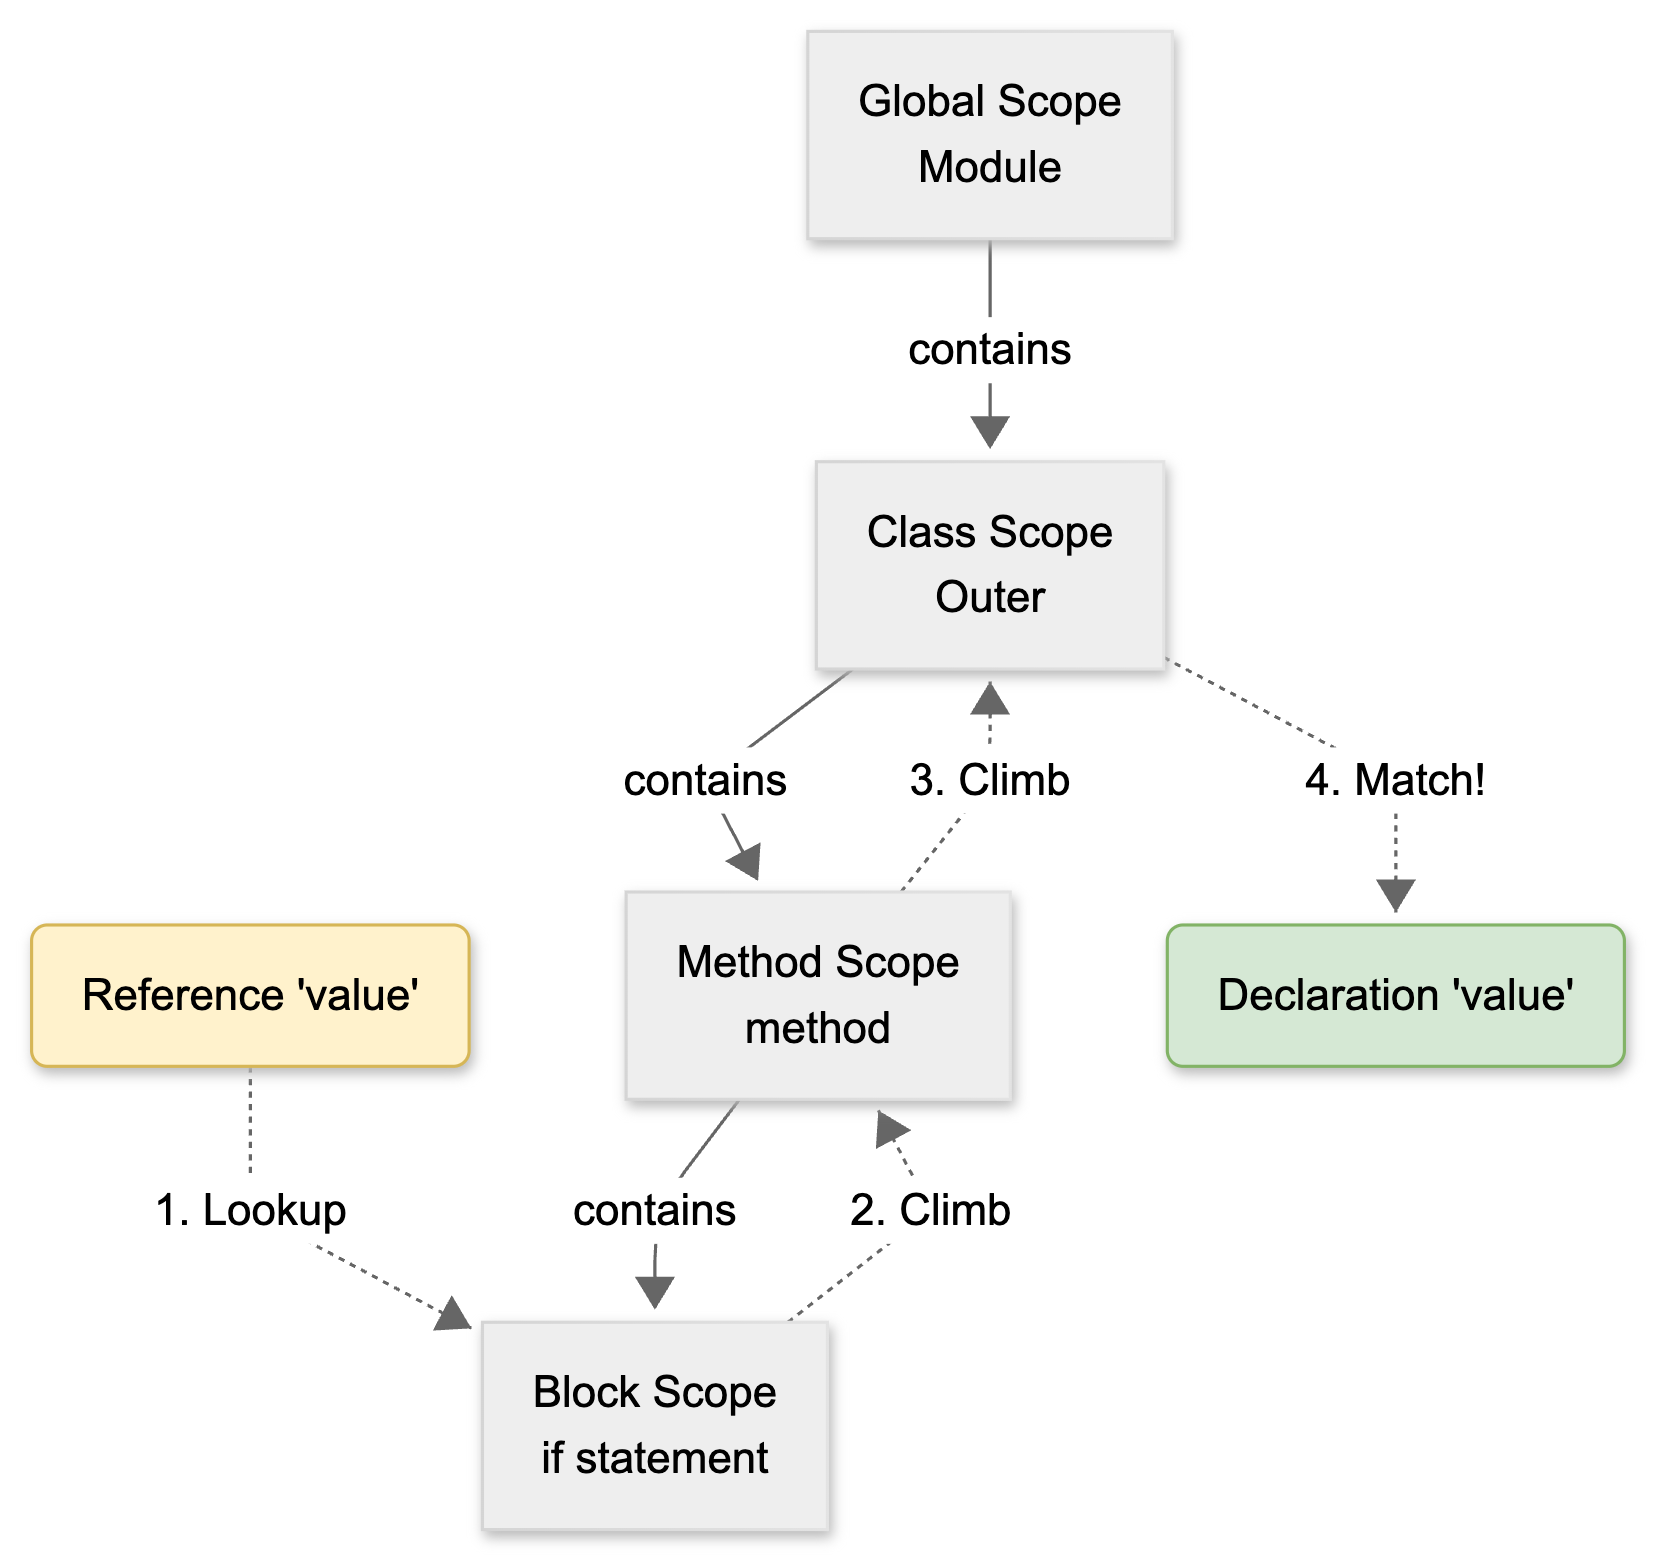
\includegraphics[width=0.6\textwidth]{images/background/scope_climbing.png}
  \caption{Visual representation of the scope climbing algorithm: the
    search starts from the inner-most block and climbs up the hierarchy
  until the identifier is found.}
  \label{fig:scope_climbing}
\end{figure}

Furthermore, different programming languages handle namespaces,
imports, and symbol resolution in drastically different ways. Because
types can reference each other cyclically or be referenced before
they are declared (forward declarations), resolving symbols in a
\textbf{single linear pass} over the code is generally impossible.

Consequently, structural extraction must be strictly
\textbf{decoupled} from semantic resolution. The syntactic phase
(Extraction) must first traverse the CST to catalog all available
declarations and record unresolved identifiers along with the exact
context and scope in which they appear. Only afterward can a
dedicated, \textbf{multi-pass resolution phase} traverse the
hierarchical scope boundaries to semantically link these identifiers
to their concrete definitions. This separation of concerns is a
central architectural decision in designing a scalable,
language-agnostic analyzer.

\subsection{Type Systems, Dynamic Typing, and Type Hints}
The complexity of name resolution is heavily influenced by the
\textbf{Type System} of the underlying language
\cite{pierce_types_2002}. In statically typed languages (such as
Java, C++, and Rust), the type of every variable, field, and method
return is explicitly declared (or rigorously inferred at compile
time). This makes static resolution deterministic: if a variable
\texttt{v} is declared as type \texttt{A}, any method call
\texttt{v.foo()} can be reliably resolved by looking up the
definition of \texttt{foo} within class \texttt{A}.

Conversely, dynamically typed languages (such as Python) utilize
\textbf{duck typing}, where variables do not possess inherent types,
and their types can change freely at runtime based on the assigned
values. In such environments, determining the target of
\texttt{v.foo()} using only static text analysis is fundamentally
ambiguous without executing the code.

To bridge this gap and enable robust static analysis in dynamically
typed environments, modern ecosystems have introduced optional static
typing mechanisms, such as \textbf{Type Hints} (e.g., Python's PEP
484 \cite{pep484}). Type hints allow developers to annotate
variables and function signatures with expected types without
altering the runtime behavior.

Consider the Python example in Listing \ref{lst:type_hints}. Without
annotations, a static analyzer cannot determine the type of the
\texttt{user} parameter, making it impossible to resolve the target of the
\texttt{user.send()} method call. By providing type hints, the parameter
is explicitly linked to the \texttt{User} class, allowing deterministic
resolution.

\begin{lstlisting}[language=Python,caption={Comparison of a Python function without and with Type Hints (PEP 484).},label={lst:type_hints}, morekeywords={User}]
# Without type hints: 'user' is opaque to static analysis
def notify(user):
    user.send("Hello") # What is 'user'? Impossible to resolve statically.

# With type hints:
from models import User

def notify(user: User) -> bool:
    user.send("Hello") # Can be deterministically resolved to User.send
    return True
\end{lstlisting}

For the purposes of this thesis, extracting architectural
dependencies from dynamically typed languages relies on a crucial
\textbf{assumption}: we assume that the source code is adequately
decorated with Type Hints. When these annotations are present, the
analyzer can treat them as pseudo-static declarations, mapping them
to the internal IR and performing deterministic name resolution
identically to statically typed languages. Without these hints,
static resolution falls back to heuristics or yields unresolved
edges, highlighting the inherent limits of analyzing dynamic
languages statically.
